%-------------------------------------------------------------------------------
\subsubsection{Système différentiel d'ordre trois} 
%-------------------------------------------------------------------------------

On considère l'équation différentielle ordinaire non-linéaire
\begin{equation} \label{eq:L3BioSUTD2E2}
\dot x = f(x) = -x^3 + 7x^2 - 15x + 8.
\end{equation}
% dans laquelle $x$ désigne la concentration d'un métabolite : \eqref{eq:L3BioSUTD2E2} modélisant l'ensemble des réactions biochimiques impliquées dans la production/dégradation de ce métabolite.

\begin{enumerate}
  \item Déterminer l'ensemble des points stationnaires de \eqref{eq:L3BioSUTD2E2}.
  \solution{On cherche les raçines de $f(x)$. 1 est une racine évidente, et, en déterminant les raçines de $x^2 - 6x + 8$, on voit que $f(x)$ se factorise en
  \begin{align*}
    f(x) & = (x-1) (x^2 - 6x + 8) = (x-1) (x - 2) (x - 4). 
  \end{align*}
  Les points stationnaires sont donc $x^*_1 = 1$, $x^*_2 = 2$ et $x^*_3 = 4$.}
  \item \'Etudier la stabilité de chacun de ces points stationnaires.
  \solution{On calcule
  $$
  f'(x) = -3 x^2 + 14x -15
  $$
  et on conclue 
  \begin{align*}
    f'(x^*_1) & = -3 < 0 & \Rightarrow \quad x^*_1 & = 1 \text{ est stable}, \\ 
    f'(x^*_2) & = + 2 > 0 & \Rightarrow \quad x^*_2 & = 2 \text{ est instable}, \\ 
    f'(x^*_3) & = -6 < 0 & \Rightarrow \quad x^*_3 & = 4 \text{ est stable}. 
  \end{align*}}
  \item Tracer le diagramme de stabilité du système.
  \solution{$$
  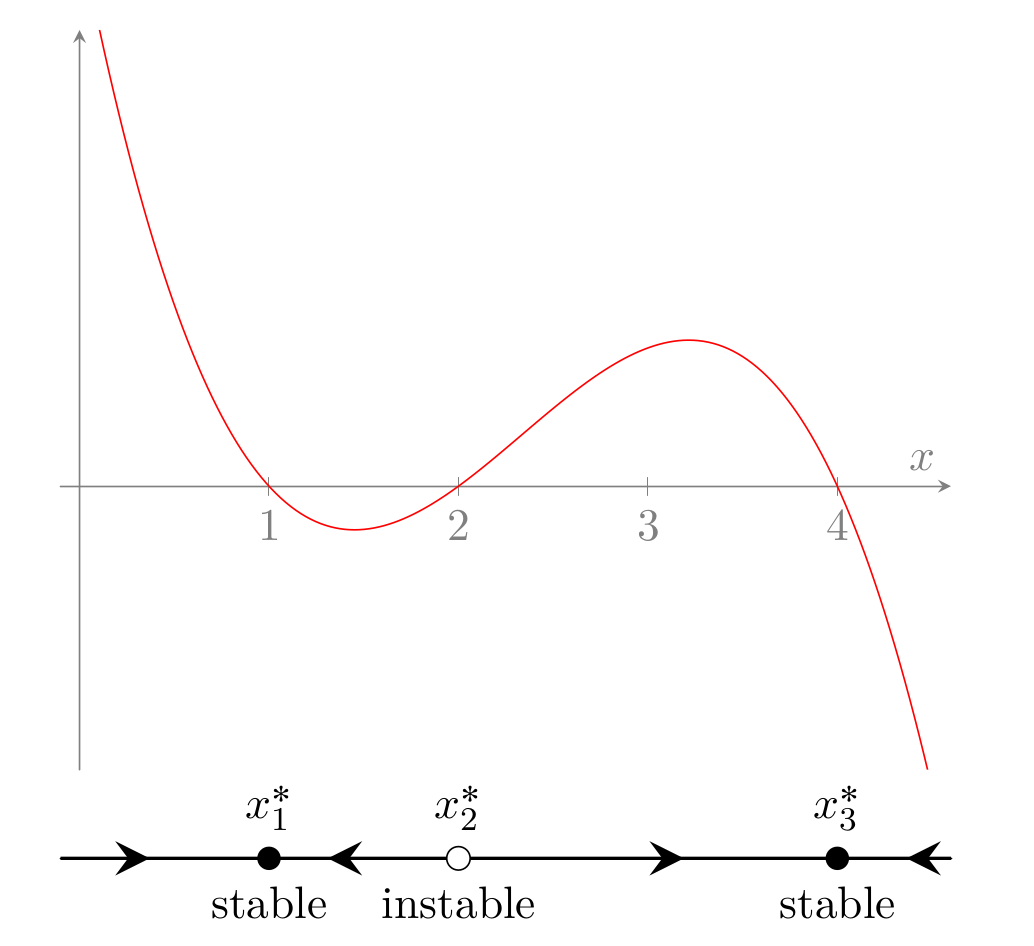
\includegraphics[width=.4\textwidth]{L3bioSU-TD2exo2}
  $$}
  \item D'un point de vue du comportement du système, quels sont les rôles respectifs de chacun des points stationnaires.
  \solution{
  \begin{itemize}
   \item $x^*_1$ et $x^*_3$ sont des équilibre stables et attracteurs vers lesquels le système tend. On perle de bistabilité.
   \item $x^*_2$ est le point critique (stationnaire mais répulsif) : la position de $x(0$ par rapport à $x^*_2$ détermine l'état final du système.
  \end{itemize}}
\end{enumerate}
